\documentclass[a4paper,14pt]{extarticle}

\usepackage[T2A]{fontenc}
\usepackage[utf8]{inputenc}
\usepackage[english,russian]{babel}
\usepackage[left=3cm, right=1.5cm, top=2cm, bottom=2cm]{geometry}
\usepackage{setspace}
\onehalfspacing%
\usepackage[center]{titlesec}
\usepackage{indentfirst}
\setlength{\parindent}{20pt}
\usepackage{fancyhdr}
\pagestyle{fancy}
\fancyhf{}
\fancyhead[C]{\thepage}
\renewcommand{\headrulewidth}{0pt}
\usepackage[normalem]{ulem}

\hyphenpenalty=0

\usepackage[acronym]{glossaries}

\usepackage{multirow}
\usepackage[hidelinks]{hyperref}

\usepackage{graphicx}
\graphicspath{{images/}}

\usepackage{miller}
\newcommand{\unit}[1]{ \ \text{#1}}
\newcommand{\degree}{^\circ}
\newcommand{\celcius}{^\circ \text{C}}
\newcommand{\YEu}{${(\text{Y}_{1-x}\text{Eu}_x)}_2\text{O}_3$}
\newcommand{\range}[2]{[#1\div#2]}

\usepackage{forloop}
\newcounter{x}
\newcommand{\Repeat}[2]{\forloop{x}{0}{\value{x} < #1}{#2}}
\newcommand{\writedate}{<<\Repeat{2}{\ldots}>>\Repeat{5}{\ldots}2025г.}

\bibliographystyle{gost-numeric.bbx}
\usepackage[backend=biber,
citestyle=gost-numeric,
bibstyle=gost-numeric,
]{biblatex}
\addbibresource{bibliography.bib}

\begin{document}
\begin{titlepage}
\thispagestyle{empty}
\begin{spacing}{1.15}
\footnotesize
\begin{center}
    МИНИСТЕРСТВО НАУКИ И ВЫСШЕГО ОБРАЗОВАНИЯ РОССИЙСКОЙ ФЕДЕРАЦИИ
    \vspace{20pt}

    ФЕДЕРАЛЬНОЕ ГОСУДАРСТВЕННОЕ АВТОНОМНОЕ ОБРАЗОВАТЕЛЬНОЕ\\
    УЧРЕЖДЕНИЕ ВЫСШЕГО ОБРАЗОВАНИЯ
    \vspace{6pt}

    «НОВОСИБИРСКИЙ НАЦИОНАЛЬНЫЙ ИССЛЕДОВАТЕЛЬСКИЙ ГОСУДАРСТВЕННЫЙ УНИВЕРСИТЕТ» (НОВОСИБИРСКИЙ ГОСУДАРСТВЕННЫЙ УНИВЕРСИТЕТ, НГУ)
    \vspace{10pt}
\end{center}
Факультет \uline{\textbf{ФИЗИЧЕСКИЙ}}
\vspace{10pt}

\noindent
Кафедра \uline{\textbf{ФИЗИЧЕСКИХ МЕТОДОВ ИССЛЕДОВАНИЯ ТВЕРДОГО ТЕЛА}}
\vspace{8mm}

\noindent
Направление подготовки \uline{\textbf{03.03.02 ФИЗИКА}}
\vspace{10pt}

\noindent
Образовательная программа: \uline{\textbf{БАКАЛАВРИАТ}}
\vspace{8mm}
\begin{center}
    \textbf{ВЫПУСКНАЯ КВАЛИФИКАЦИОННАЯ РАБОТА}

    \textbf{(научно-исследовательский формат)}
    \vspace{8mm}

    \uline{\hfill Кудрявцева Артема Леонидовича \hfill}

    $_\text{(Фамилия, Имя, Отчество автора)}$
    \vspace{8mm}
\end{center}
Тема работы \uline{Разработка прецизионного метода определения параметров элементарной ячейки для монокристального дифрактометра, оснащенного двумерным детектором \hfill}
\vfill

\noindent
\textbf{<<К защите допущена>>}

\noindent
Заведующий кафедрой \hfill \textbf{Научный руководитель}
\vspace{10pt}

\noindent
д.~ф.-м.~н., профессор \hfill д.~ф.-м.~н., профессор
\vspace{10pt}

\noindent
г.~н.~с. ИК СО РАН \hfill г.~н.~с. ИНХ СО РАН
\vspace{10pt}

\noindent
Цыбуля~С.В./\Repeat{4}{\ldots}\hfillГромилов~С.А./\Repeat{4}{\ldots}

\noindent
$_\text{(фамилия И., О.) / (подпись, МП)}$ \hfill $_\text{(фамилия И., О.) / (подпись, МП)}$
\vspace{10pt}

\noindent
\writedate\hfill\writedate{}
\vspace{8mm}

\hfill Дата защиты:\writedate{}
\vspace{8mm}

\begin{center}
    Новосибирск, 2025
\end{center}

\end{spacing}
\end{titlepage}
\newpage
\tableofcontents
\newpage
\section{Введение}

\subsection{Параметры элементарной ячейки}

Параметры элементарной ячейки (ПЭЯ) --- величины, определяющие метрику кристаллической решетки.
Они являются одними из основных характеристик кристаллов.
В общем случае, их представляют в виде шести различных вещественных величин: трех длин, соответствующих периодам главных направлений кристаллической решетки $(a, b, c)$, и трех углов между этими направлениями $(\alpha, \beta, \gamma)$.
Однако, благодаря симметрии кристалла, общее число независимых параметров может быть меньше: минимум одна длина $a$ в случае кубической сингонии.

На ПЭЯ кристалла влияет множество различных факторов, таких как: состав, структура, дефектность, температура, давление и другие.
Это позволяет по изменению ПЭЯ кристалла косвенно их отслеживать.
В общем случае, при значительной разнице в ПЭЯ можно говорить, что кристаллы заметно отличаются, а при достаточной точности измерений и знании того, что может отличаться --- дать количественную оценку изменения этих величин.

Однако, при небольшом их изменении, разница в ПЭЯ крайне мала.
Так, например, температурные коэффициенты расширения большинства материалов порядка $10^{-5} \unit{K}^{-1}$.
Для твердых растворов же, относительная разница значений ПЭЯ для соответствующих чистых веществ порядка $10^{-2}$, и, при изменении мольной доли на $10^{-3}$, относительное изменение ПЭЯ уже составит порядка $10^{-5}$.
Похожим образом ситуация обстоит и с остальными величинами.
Поэтому при использовании ПЭЯ для измерения косвенно связанных с ним характеристик, необходима высокая точность измерений.

Хотя, технически правильнее будет говорить не о точности, а о <<прецизионности>> измерений, от английского \textit{precision}.
В работе эти термины будут отличаться, и разница в них будет заключается в разных ошибках, которым они соответствуют.
Высокая точность будет означать, что полученные значения мало отличаются от истинного значения, а высокая прецизионность --- то, что полученные значения будут мало отличаться друг от друга.
Можно сказать, что для точных результатов систематическая ошибка значительно меньше случайной, а для прецизионности наоборот --- случайная меньше систематической.
В описанном выше случае измерения величин, слабо влияющих на ПЭЯ, систематическая ошибка практически не будет влиять на получаемые результаты, ведь обычно приходится оценивать относительную разницу величины ПЭЯ.

\subsection{Методы измерения}

Наконец, стоит рассказать о самих методах измерения ПЭЯ.
Самыми эффективными и распространенными являются различные дифракционные методы: рентгеновские, нейтронные и электронные.
Среди них самым доступным и неприхотливым является именно рентгеновская дифракция, и только она будет рассматриваться в дальнейшем.
В любой дифракции, тем не менее, основным уравнением, позволяющим, зная длину волны $\lambda$ излучения и угол дифракции $2\theta$, получить межплоскостные расстояния в кристалле $d$ является уравнение Вульфа-Брэгга~(\ref{eq:bragg}).
\begin{equation} \label{eq:bragg} 
    2 d \sin{\theta} = \lambda
\end{equation}

Установками, на которых она реализуется являются обычно лабораторные дифрактометры и специализированные станции синхротронного излучения (СИ).
Между ними, конечно, есть принципиальная разница в источнике излучения, но общая схема установки у них одинаковая.
Они состоят из:
\begin{itemize}
    \item Источника излучения
    \item Исследуемого образца
    \item Детектора излучения
\end{itemize}
В добавок к этому, каждый из этих компонентов может быть механизирован, то есть для них может регулироваться положение и ориентация в пространстве.
В качестве примера, лабораторные монокристальные дифрактометры обычно оснащаются гониометром, с помощью которого возможно точное вращение кристалла.
Так же может быть и механизирован и детектор: может регулироваться расстояние между ним и образцом, а также сам детектор обычно может вращаться вокруг образца.
Перемещение же источника возможно только для рентгеновских трубок, и это обычно реализуется в порошковых дифрактометрах.

Рентгеновские дифракционные методы отличаются между собой, и один из способов их классификации --- по виду образца: монокристальные, поликристальные, порошковые, тонкопленочные и другие.
Стандартным способом точного и воспроизводимого измерения ПЭЯ сейчас является порошковая дифракция, тогда как монокристальная используется в основном для проведения рентгеноструктурного анализа.
Может показаться странным, но данные о ПЭЯ, получаемые сейчас из рентгеноструктурного анализа по монокристальной дифракции часто являются менее достоверными и воспроизводимыми, чем порошковые данные~\cite{Dudka:2017}.
Это связано, в основном, с использованием двумерных детекторов вместо точечных.

\subsection{Двумерные детекторы}

Двумерные или, по-другому, матричные детекторы используют полупроводники для регистрации рентгеновских квантов.
Есть три основных типа таких детекторов: CCD, CMOS и HPAD~\cite{Alle:2016}.

CCD, или \textit{charge-coupled device} --- это прямые аналоги матриц, используемых для съемки в видимом диапазоне.
Рентгеновские кванты попадая на сцинтиллятор детектора преобразуются в фотоны, которые затем преобразуются фотодиодом в электроны и собираются в потенциальные ямы, называемые пикселями детектора.
Затем этот заряд автоматически измеряется электроникой и получается двумерное изображение, на котором интенсивность каждого пикселя напрямую связана с зарядом, накопленном в яме.

CMOS, или \textit{complementary metal-oxide-semiconductor} --- это по-сути усовершенствованная версия CCD-матрицы.
Главное отличие их в том, что в CMOS рядом с каждым пикселем детектора располагается небольшая электронная схема, обрабатывающая получаемый сигнал, усиливая его и нормализуя.
Это делает данные более достоверными, уменьшая ошибки, но увеличивает размеры пикселя, а также уменьшает активную площадь потенциальной ямы для электроном, что в свою очередь уменьшая общую чувствительность детектора.

HPAD, или \textit{hybrid pixel array detector} принципиально отличается от предыдущих двух.
Они основываются на технологии регистрации высокоэнергетических фотонов в физике высоких энергий.
По-сути это матрица из полупроводниковых счетчиков рентгеновских фотонов.
В каждом таком счетчике каждый фотон напрямую в полупроводнике преобразуется в электрон-дырочные пары без промежуточного преобразования в фотоны видимого диапазона.
Такие детекторы точнее, быстрее и эффективнее тех, что использую сцинтилляторы.

\subsection{Мотивация разработки методики}

Теперь учитывая то, что технологии детектирования рентгеновского излучения стремительно развились по сравнению с точечными детекторами, а точность определения ПЭЯ оставляет желать лучшего, то значит, что проблема монокристальной дифракции может заключаться в плохой технике эксперимента или обработке данных.
Матричные детекторы позволяют значительно увеличить объемы собираемых данных, и за короткое время можно <<просканировать>> все обратное пространство кристалла.
Но в то же время качество снимаемых рефлексов при этом неумолимо страдает.
После съемки полученные пики как-то обрабатываются программами, работающими как <<черный ящик>>, и они же выдают значения ПЭЯ.
В процессе, могут уточняться инструментальные параметры прибора, и весь набор координат пиков по-сути аппроксимируется с помощью метода наименьших квадратов (МНК).
Такой подход, и дает плохую точность определения ПЭЯ при монокристальной дифракции и использовании двумерных детекторов.

Для точного определения межатомных расстояний после расшифровки структуры кристалла, важны не только относительные координаты атомов в ячейке $(x, y, z)$, но и ПЭЯ, причем с относительной точностью не хуже чем относительные координаты атомов.
Поэтому метод, который бы позволил без больших затрат точно определять ПЭЯ на первом этапе рентгеноструктурного анализа (РСтА) с тем же образцом и на той же установке позволил бы улучшить его результаты.

Также точный метод определения ПЭЯ можно использовать и для калибровки других дифракционных установок.
Хорошо измерив ПЭЯ на одном приборе, можно использовать тот же кристалл на другом приборе для его калибровки.
Впоследствии это позволит более объективно сравнивать результаты, получаемые на двух разных установках.

Все написанное выше является является мотивацией к теме работы --- разработке прецизионного метода определения ПЭЯ для малых монокристаллов на установках, оснащенных матричным детектором.
Малость монокристалла возникает из-за требования схожести образца с тем, что используется в РСтА.

\section{Обзор методов}

Перед разработкой самой методики были изучены обзорные статьи~\cite{Lider:2020,Galdecka:2006} с целью поиска базового метода, на котором можно будет построить желаемую методику.
В указанных обзорах приводятся различные рентгеновские дифракционные методы измерения и уточнения ПЭЯ.
Их все можно разбить на три группы:
\begin{itemize}
    \item Полихроматические методы (метод Лауэ)
    \item Методы с монохроматичным, но широко расходящимся пучком (метод косселевских проекций)
    \item Методы с монохроматичным и коллимированным пучком.
\end{itemize}
Среди них выбирался тот, который можно адаптировать под стандартный лабораторный монокристальный дифрактометр.
Такой дифрактометр предполагается оснащенным:
\begin{itemize}
    \item Рентгеновской трубкой с хорошо коллимированным пучком
    \item Как минимум однокружным гониометром для образца
    \item Матричным детектором с регулируемым углом поворота вокруг образца
\end{itemize}
Таким образом, в рассмотрении остаются только методы, использующие монохроматическое и коллимированное излучение, так как используемое в лабораторных дифрактометрах характеристическое излучение можно считать монохроматическим, относительно фонового тормозного.

\subsection{Метод Бонда}

В первую очередь из этих методов выделяется метод Бонда.
Он является простым, безэталонным, универсальным, и позволяющим получить хорошую точность, вплоть до $10^{-6}$.

В оригинальном исполнении схема Бонда~\cite{Bond:1960} представляет собой однокристальный спектрометр.
В качестве источника используется микрофокусная рентгеновская трубка с коллиматором в виде пары пластин дающих расходимость первичного пучка около $0.8'$.
Кристалл --- это ориентированная полированная пластина из монокристаллического кремния, значительно превосходящая размерами первичный пучок.
Для поддержания постоянной температуры в $24.7\celcius$ образца при этом используется водяное охлаждение.
Кристалл был закреплен на гониометре, позволяющим регулировать угол наклона кристалла и вращать его в одной плоскости $\omega$ с точностью до $1''$.
В качестве детекторов использовались два счетчика гейгера, которые считаются точечными детекторами.
Они могли вращаться в той же плоскости, что и кристалл.

Само измерение ПЭЯ в схеме Бонда выглядит так:
\begin{enumerate}
    \item Выбирается плоскость кристалла, отражение от которой будет измеряться
    \item Отражающая плоскость выставляется перпендикулярно первичному пучку
    \item Детектор устанавливается под углом, чтобы зарегистрировать отражение от плоскости
    \item Измеряется зависимость интенсивности на детекторе от угла поворота $\omega$ кристалла вблизи отражающего положения (кривая качания)
    \item Из полученной зависимости определяется угол $\omega_1$ при котором достигается максимум интенсивности на детекторе
    \item Предыдущие три шага повторяются для симметричного положения детектора и определяется второй угол $\omega_2$
    \item Угол дифракции вычисляется как $2\theta=180\degree-|\omega_1-\omega_2|$
\end{enumerate}
Затем уже значения межплоскостных расстояний вычисляются из уравнения Вульфа-Брэгга~(\ref{eq:bragg}), и, зная индексы Миллера отражающих плоскостей и сингонию кристалла, это позволяет вычислить наконец и значения ПЭЯ.

При определении угла $2\theta$ по такой схеме исключаются ошибки, связанные с:
\begin{itemize}
    \item Смещением образца (эксцентриситетом)
    \item Поглощением в кристалле
    \item Положением нуля гониометра
\end{itemize}
Другие же ошибки имеют незначительное влияние и для них есть выражения, позволяющие вводить поправки для их учета.
Список источников этих ошибок:
\begin{itemize}
    \item Неточное выведение отражающей плоскости параллельно оси вращения $\omega$
    \item Расходимость первичного пучка
    \item Отклонение первичного пучка от плоскости $\omega$
    \item Преломление в кристалле
    \item Фактор Лоренца-поляризации
    \item Ошибка измерения угла
\end{itemize}

В оригинальной работе Бонда ему удалось достигнуть относительной погрешности определения ПЭЯ около нескольких частей на миллион, то есть порядка $10^{-6}$.

\subsection{Модификации метода Бонда}

Схема Бонда была адаптирована и для изучения малых монокристаллов~\cite{Hubbard:1976,Ponomarev:1969}.
Для этого было предложено дополнительно измерять угол отражения от фриделевской пары выбранной плоскости.
Углы $\omega$ для фриделевской пары плоскостей отличаются в таком случае на $180\degree$, и это позволяет уменьшить ошибку калибровки гониометра.
Остальные ошибки уменьшаются за счет учета ассиметричности кривой качания.
Она смещает измеряемое значение угла $\omega$, но при использовании фриделевской пары, это смещение в оказывается преимущественно направлено в разные стороны.
Таким образом, полусумма углов $\omega$ для фриделевской пары плоскостей позволяет в среднем уменьшить погрешность определения ПЭЯ.

Для трехкружного гониометра возможно использование методики измерения от одной плоскости уже для 8 различных углов гониометра~\cite{King:1979}.
В такой схеме можно учесть еще больше ошибок, связанных со смещением образца от точки сведения осей гониометра, а также она позволяет определить нулевые положения гониометра.
Для реализации этого метода даже была написана специальная программа, которые позволяют калибровать дифрактометры с трехкружными гониометрами и точечными детекторами~\cite{Angel:2011}.

\subsection{Метод щелей Соллера}

В работе~\cite{Berger:1984} предлагается метод, использующий всего одно отражающее положение кристалла, но при этом получаемая точность оказывается не хуже чем в методе Бонда, то есть порядка $10^{-6}$.
Угол дифракции же в нем измеряется с помощью щелей Соллера.

В этом методе сначала кристалл и детектор выводятся в отражающее положение, при котором наблюдается максимальная интенсивность дифрагированного луча.
После этого на гониометр устанавливаются щели Соллера, и измеряется угол между их положениями на гониометре, в которых наблюдается максимальная интенсивность.

Из-за использования щелей Соллера, этот метод оказывается невосприимчивым к центрировке образца, и в нем можно использовать источник с большой расходимостью.
По сравнению с методом Бонда он оказывается более сложным, и требует больше специального оборудования для реализации.

\subsection{Метод четырехкристального спектрометра}

Похожий метод измерения угла~\cite{Fewster:1989} использует два кристалла для монохроматизации первичного пучка и один на дифрагированном пучке.
Этот метод, так же как и использующий щели Соллера, невосприимчив к центрировке образца.
Из его недостатков можно отметить, что он требует серьезной модификации установки и тщательной юстировки.

\subsection{Метод компланарных рефлексов}

Этот метод~\cite{Isomae:1976} возможен только для кристаллов, в которых угол между определенными плоскостями однозначно определяется индексами Миллера и не зависит от экспериментально определенных параметров.
При этом измеряется малый угол, на который нужно повернуть кристалл, чтобы вместо отражения от одной плоскости, появилось отражение от второй.
Из-за малого угла поворота, условия съемки практически неизменны для двух отражающих положений, что позволяет свести ошибки, связанные с этим к минимуму.
Этот метод также обладает высокой точностью, на уровне $10^{-6}$.

\subsection{Метод многолучевой дифракции}

Многолучевая дифракция возникает, когда две или более плоскостей оказываются в отражающем положении одновременно.
При этом возможно наблюдение рефлексов, запрещенных кинематической теорией дифракции.
Такое явление впервые наблюдалось Реннингером~\cite{Renninger:1937} и было названо им \textit{Umweganregung} или <<окольным возбуждением>>.
Пики, возникающие в при многолучевой дифракции, получаются более узкими, чем обычные, и поэтому их положение можно измерять более точно.
Но точность такого метода в итоге оказывается не сильно лучше того же метода Бонда: всего лишь на уровне $10^{-5} - 10^{-6}$.

\subsection{Методы эталонов}

Методы эталонов предполагают определение межплоскостных расстояний опираясь не на известную длину волны, а на хорошо известные ПЭЯ эталонного кристалла.
Вообще, эталоны могу использоваться неявно для калибровки дифрактометра, или явно в виде дополнительных, используемых одновременно с образцом кристаллов.
Может быть применен внутренний эталон как в порошковой дифракции, где в исследуемый образец добавляются кристаллы эталонного и снимается дифракционная картина их обоих одновременно.
Использование эталонов само по себе не является конкретной схемой эксперимента, а говорит о внедрении в него дополнительного источника информации.
Явное использование эталонов для измерения ПЭЯ никак не будет использоваться для разработки методики, так как это достаточно сложно и не подходит под поставленные условия.

\subsection{Выбор метода}

Среди всех перечисленных методов в итоге был выбран самый первый --- метод Бонда.
Его простота и универсальность оказываются очень привлекательными и поэтому должны сделать итоговую методику более доступной.

\section{Экспериментальная часть}
\subsection{Описание установки}
Рентгенографические эксперименты проводились на монокристальном дифрактометре Bruker D8 Venture.
\begin{itemize}
    \item Микрофокусная трубка Incoatec $I \mu S \ 3.0$
    \begin{itemize}
        \item $\text{Cu} K\alpha$ и $\text{Mo} K\alpha$ излучение
        \item Монохроматизация и коллимация с помощью многослойных зеркал Монтеля
        \begin{itemize}
            \item Диаметр пучка $110\unit{мкм}$
            \item Расходимость пучка $0.3\degree$
        \end{itemize}
    \end{itemize}
    \item Двумерный детектором PHOTON III
    \begin{itemize}
        \item Разрешение $768 \times 1024$ пикселей
        \item Размер пикселя $135 \times 135\unit{мкм}^2$
        \item Ручная установка расстояния до образца
    \end{itemize}
    \item Трехкружный гониометр FIXED-CHI
    \begin{itemize}
        \item Угол $\chi$ фиксирован и равен $54.7112\degree$
        \item Паспортная воспроизводимость установки углов $0.0001\degree$
        \item Паспортная точность установки углов не указана, но согласно результатам измерения эталонного образца на порошковом дифрактометре Bruker D8 Advance, оснащенном аналогичным гониометром, она не хуже $0.005\degree$
    \end{itemize}
    \item Температурная приставка Oxford Cryostream 800Plus
    \begin{itemize}
            \item Стабильность поддержания температуры $0.2\unit{К}$
    \end{itemize}
    \item Управление прибором средствами программного пакета APEX3~\cite{Bruker:2019}.
\end{itemize}
Необходимо отметить, что из-за расположения трубок, область доступных углов для детектора оказывается ограниченной.
Для использовавшегося расстояния от образца до детектора около $130\unit{мм}$, угол $2\theta_D$ не мог превосходить примерно $100\degree$.

\begin{figure}[ht!]\label{fig:D8_photo}
    \centering
    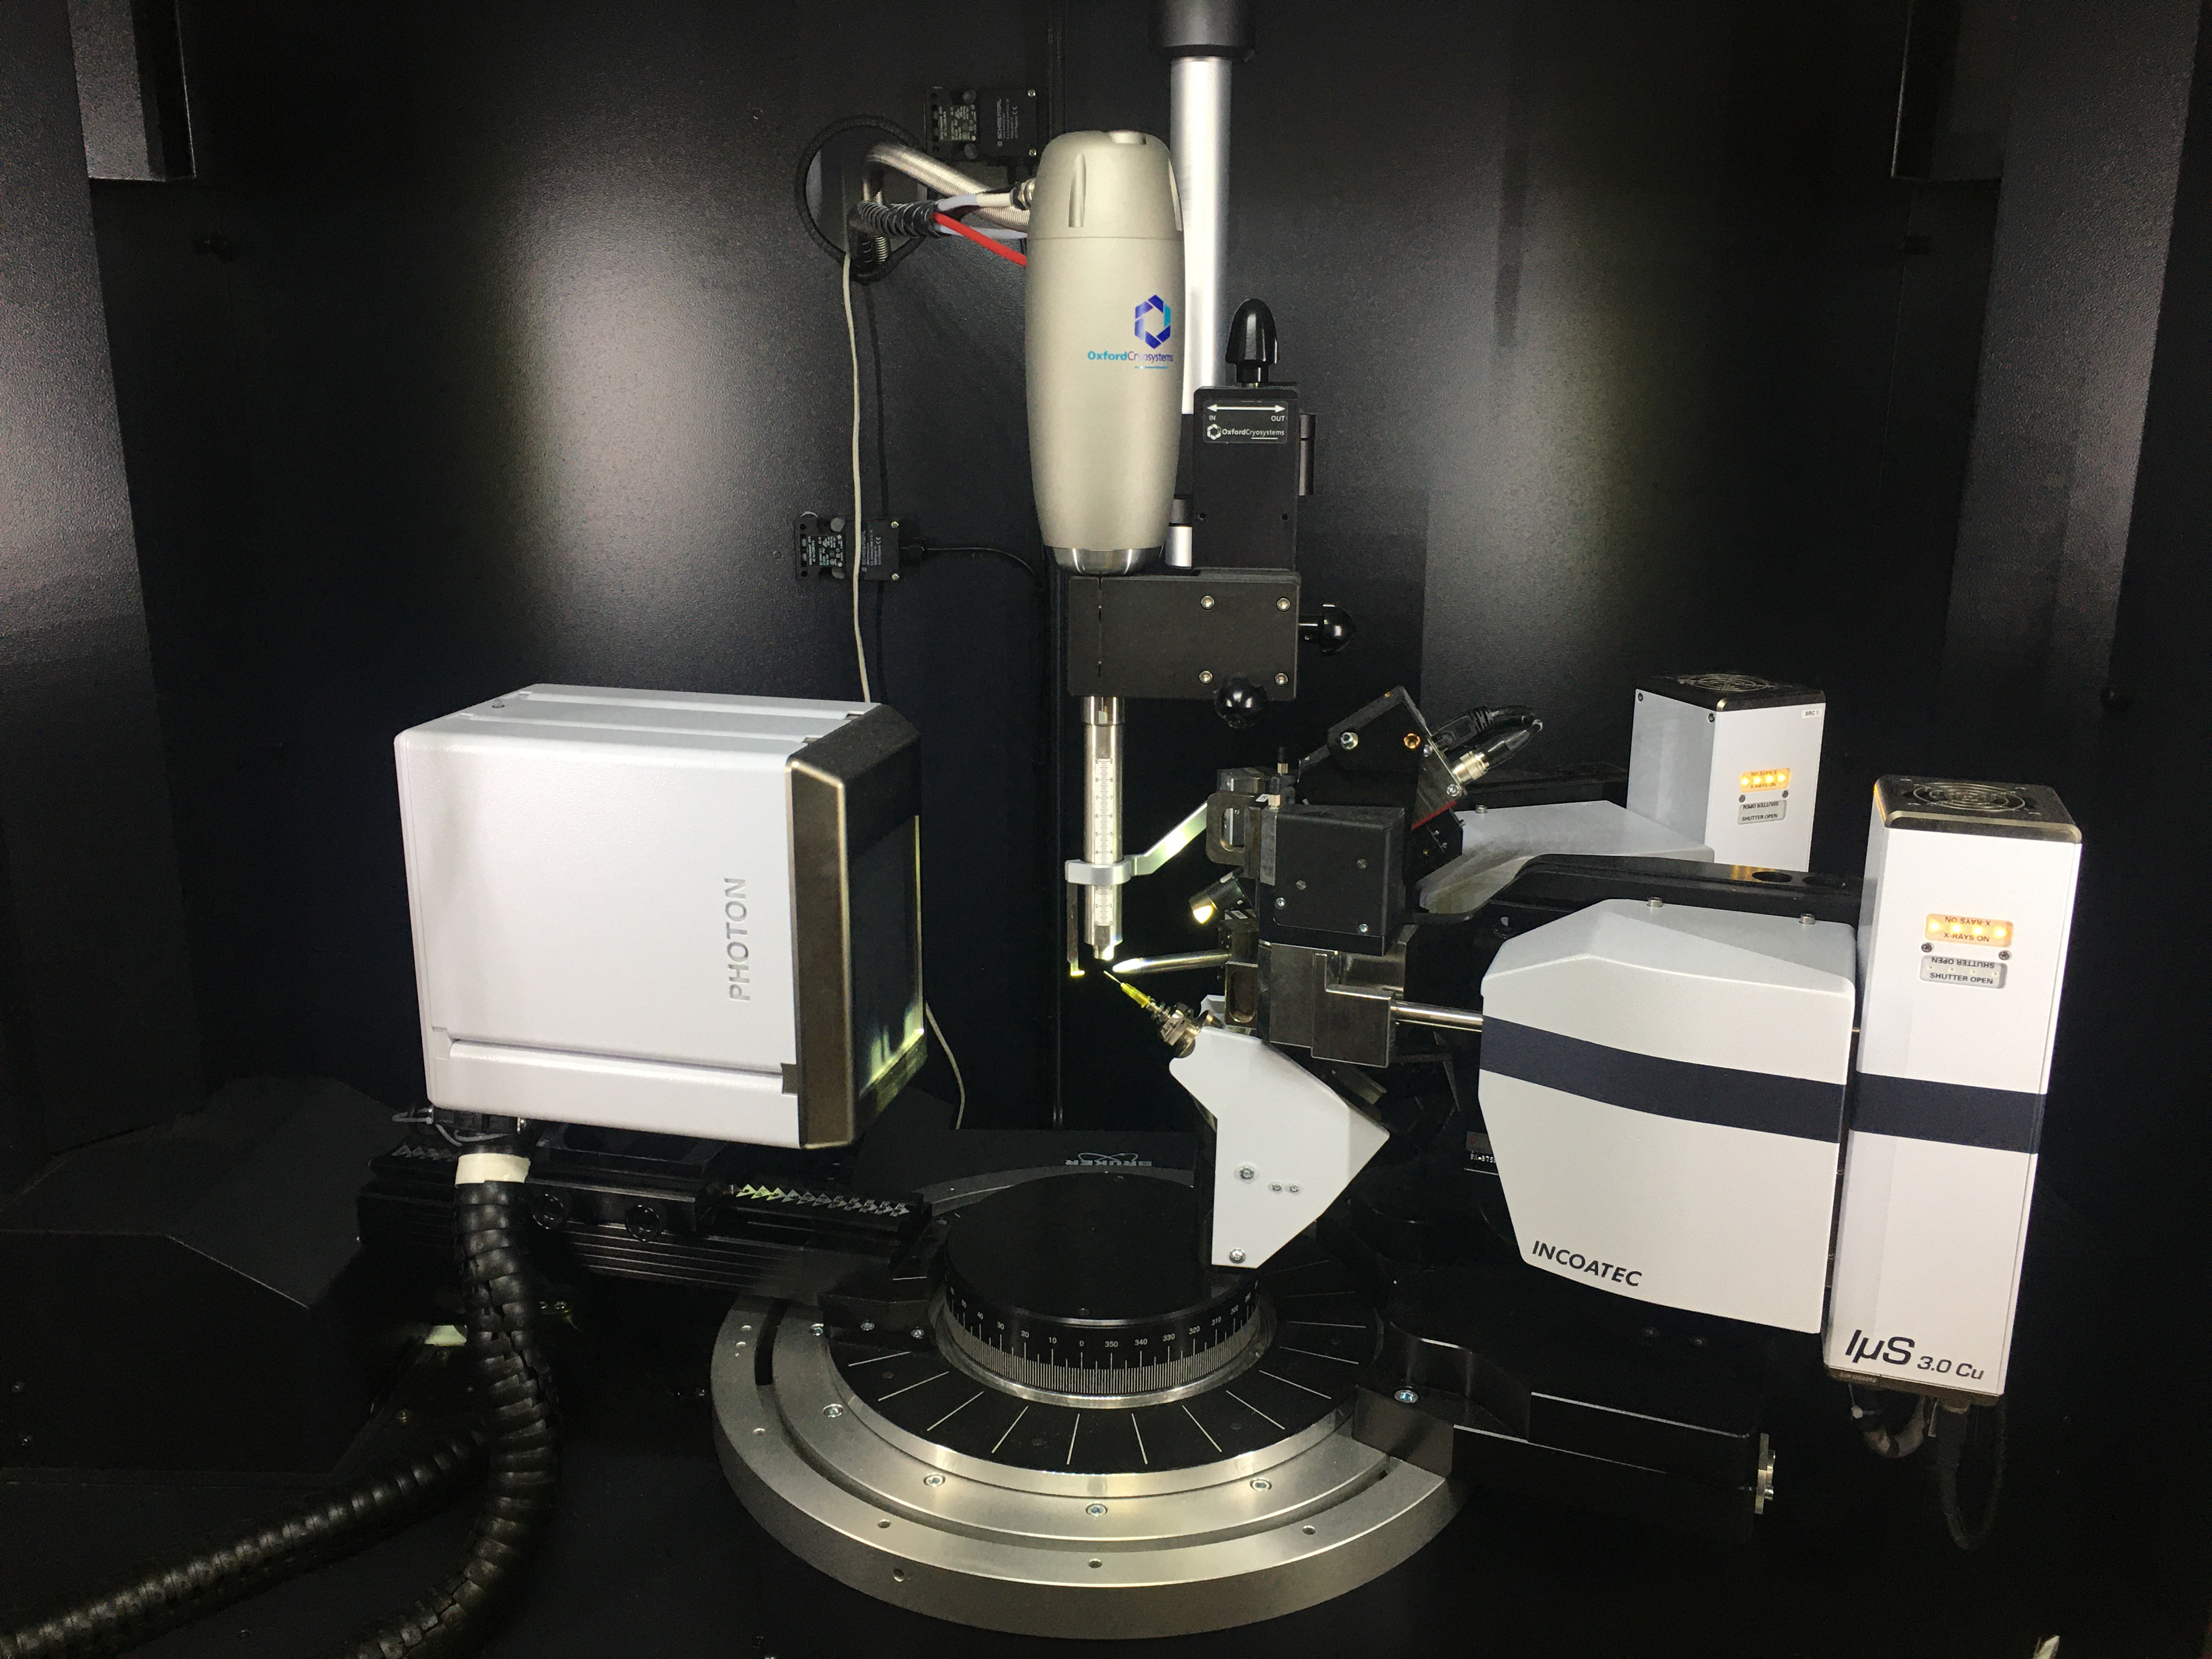
\includegraphics[width=0.8\textwidth]{d8_3.jpeg}
    \caption{Фото установки}
\end{figure}

Значения характеристических длин волн, использованных в этой работе приведены в таблице~\ref{tab:wavelengths}.
\begin{table}[ht!]\label{tab:wavelengths}
    \centering
    \begin{tabular}{|c|c|c|}  
        \hline
        Анод & $K\alpha_1,\unit{\AA}$ & $K\alpha_2,\unit{\AA}$ \\
        \hline
        Cu~\cite{Holzer:1997} & 1.54059290 (50) & 1.54442740 (50) \\
        Mo~\cite{Deslattes:1985} & 0.70931715 (41) & 0.713607 (12) \\
        \hline
    \end{tabular}
    \caption{Использовавшиеся значения характеристических длин волн}
\end{table}
\subsection{Исследуемые образцы}
Для определения точности методики были использованы эталонные монокристаллы Si и Ge.

Изученный монокристалл Si имел линейные размеры примерно $50 \unit{мкм}$.
Он является осколком кристалла, который ранее был исследован на однокристальном спектрометре~\cite{Lisoivan:1982}.
Значение $a = 5.430933(12)\unit{\AA}$ там было получено с использованием значение длины волны $\lambda \text{Cu} K \alpha_1 = 1.540562\unit{\AA}$.
При пересчете на более точное значение из таблицы~\ref{tab:wavelengths}, эталонное значение ПЭЯ для Si
\[ a_\text{Si} = 5.431042 (12)\unit{\AA}. \]

Изученный монокристалл Ge также был размером около $50 \unit{мкм}$.
ПЭЯ Ge уточняли несколько раз методами однокристального спектрометра, многократных отражений и многолучевой дифракции: сводка данных приведена в~\cite{Lisoivan:1982}.
Значения ПЭЯ Ge лежат в интервале от $5.65776 (2) \unit{\AA}$ до $5.657837 (15) \unit{\AA}$.
Из них было выбрано значение $a = 5.657772 (10) \unit{\AA}$~\cite{Cooper:1962}, так как оно оказывается наиболее близким к среднему.
Пересчет с использованием более точного значения длины волны дает
\[ a_\text{Ge} = 5.657885 (10)\unit{\AA} \]

Также с целью определения однородности продукта синтеза и значения мольной доли $x$ был изучен твердый раствор \YEu.
Для этого было отобрано 5 различных монокристаллов.
Для каждого из них был проведен РСтА и измерение ПЭЯ по разработанной методике.

\subsection{Описание методики}

Первое описание методики дано в статье~\cite{Kudryavtsev:2024:YEu}.
Общая схема проведения измерений выглядит примерно так:
\begin{enumerate}
    \item Отбор монокристалла
    \item Предварительная съемка
    \item Выбор рефлекса
    \item Съемка рефлекса
    \item Обработка профилей
    \item Расчет межплоскостного расстояния
\end{enumerate}
\subsubsection{Отбор монокристалла}
Отбор монокристалла проводится так же, как и для РСтА.
Монокристалл выбирается так, чтобы не превосходить размера первичного пучка.
В нашем случае оптимальный размер равен приблизительно 50~мкм.
\subsubsection{Предварительная съемка}
Предварительная съемка проводится с целью определения ориентации кристалла, его дифракционного класса и получения данных об интенсивности рефлексов.

Сама съемка состоит серии полных сканирований при вращении вокруг оси $\varphi$ с шагом $0.5\degree$ для при фиксированном угле $\omega$.
Три таких сканирования выполняются при углах детектора $2\theta_D = -45\degree, 0\degree, 45\degree$ при фиксированном расстоянии до образца $D \approx 70\unit{мм}$.

Обработка снимков и получение ориентации производится в программе APEX3.
На выходе программы получается файл формата p4p, где информация об ориентации кристалла содержится в виде UB матрицы~\cite{Busing:1967}.
\subsubsection{Выбор рефлекса}
Выбор рефлекса для съемки происходит так, чтобы погрешность измерений была минимальной.
Основными критериями в таком случае оказываются наибольшие угол $2\theta$ и интенсивность рефлекса.
При этом необходимо учитывать геометрию установки, так как не все рефлексы оказывается возможно вывести в отражающее положение для двух симметричных положений в экваториальной плоскости.

Средствами программы APEX3 производить такой перебор рефлексов неэффективно и крайне проблематично, так как программа рассчитывает для одного рефлекса максимум только одну пару углов $(\varphi, \omega)$ из двух возможных в общем случае.
Поэтому была специально написана программа~\cite{Kudryavtsev:2024:eccentr} для перебора всех рефлексов, расчета для них углов гониометра и отбора случаев когда в оказывается возможным вывести рефлекс в два симметричных положения, а также когда доступна для выведения и его фриделевская пара.

Программа позволяет находить среди множества плоскостей, связанных симметрией такие, которые можно вывести в отражающее положение хотя бы при одном (из двух симметричных) положений детектора.
Для этого используется информация о текущей ориентации кристалла на гониометре, т.е. p4p-файл, в котором находится матрица ориентации UB и предварительные значения ПЭЯ.
Используя известную длину волны, размеры пикселя, расстояние до детектора, и другие неизменные параметры прибора, программа вычисляет углы гониометра $(\varphi, \omega)$, необходимые для выведения каждой плоскости в отражающее положение на экваториальную плоскость.
В каждом случае проверяются геометрические ограничения прибора.
Полученная информация для всех подходящих рефлексов собирается в таблицу Excel, ее можно проанализировать и провести отбор.
\subsubsection{Съемка рефлекса}
Съемка рефлекса представляет собой сканирование при вращении вокруг оси $\omega$ в диапазоне $\pm 2\degree$ относительно рассчитанного значения $\omega$ для отражающего положения.
Время съемки выставлялось таким, чтобы максимум на профиле пика составлял не менее 10000~имп.

В программе APEX3 невозможно выставить время съемки больше 10~мин., поэтому для достижения последнего условия производились несколько одинаковых съемок по 10~мин. пока не будет достигнута требуемая интенсивность.
\subsubsection{Обработка профилей}
Обработка профилей состоит из нескольких этапов, по завершению которых можно рассчитать межплоскостное расстояние.
Реализована она была тоже в виде программы~\cite{Kudryavtsev:2024:eccentr}.

На входе она использует p4p-файл и информацию о примерном положении центра детектора (результат юстировки, прямое определение, калибровка).
Из экспериментального фрейма вырезается центральная область $X = \pm 30\unit{пикс.}, Y = \pm 15\unit{пикс.}$, в которой, исходя из условия $2\theta_D \approx 2\theta$, должен находиться искомый рефлекс.
Медианное значение интенсивности принимается за начальное значение фона.
Пиксели с интенсивностью больше заранее заданной принимаются за "горячие пиксели" и их значения приравниваются среднему значению по 8 соседним пикселям.
После учета горячих пикселей максимум интенсивности в выбранной области назначается примерным положением $K\alpha_1$--составляющей.
Далее, исходя из значений $D$ и $2\theta$ рассчитывается положение $K\alpha_1$--составляющей и обе точки смещаются так, чтобы теоретическое положение $K\alpha_1$ совпадало с координатами найденного максимума интенсивности.
Аппроксимация дублета проводится двумя независимыми  функциями 2D-Gauss, т.е. без закрепления междублетного расстояния и соотношения интенсивностей составляющих $2/1$.
Направлениями главных осей берутся вдоль координат детектора $X$ и $Y$ детектора.
В наших экспериментах именно функция 2D-Gauss наиболее хорошо описывала форму пика при минимальном числе уточняемых параметров: координаты максимума, полуширины (ширина на половине высоты, FWHM) в направлениях $X$ и $Y$, и интегральная интенсивность.
\subsubsection{Рассчет межплоскостного расстояния}
Для достаточно малой разницы координат рефлексов искомый угол дифракции можно рассчитать по формуле
\begin{equation} \label{eq:bond2}
    2\theta = 2\theta_D - \frac{\gamma}{2} (X_{+} - X_{-}),
\end{equation}
где $\gamma$ --- угловой размер пикселя в точке детектирования рефлекса, $X_{-}, X_{+}$ --- координаты рефлексов при отрицательном и положительном углах детектора.
В формуле $2\theta_D$ предполагается положительным.
Знак перед разницей координат рефлексов зависит от направления координаты $X$ детектора и направлением положительного вращения детектора вокруг оси $2\theta_D$.
Если они направлены в разные стороны, то знак ``$-$'', если в одну, то ``$+$''.
В нашей установке направления выбраны так, что перед разницей должен быть ``$-$''.
\subsection{Учет эксцентриситета}
Дополнительная съемка фриделевских пар позволяет учитывать эффект смещения кристалла при вращении вокруг оси $\omega$.
Так как рефлекс при съемке выводится в экваториальную плоскость, то угол $\omega$ для фриделевской пары изначального рефлекса отличается на $180\degree$.
Так как при повороте на $180\degree$ положение кристалла как бы отражается относительно оси $\omega$, то среднее значение координат рефлексов в этих двух положения будет соответствовать положению кристалла ровно на оси $\omega$~\ref{fig:eccentr}.

\begin{figure}[ht!]
    \centering
    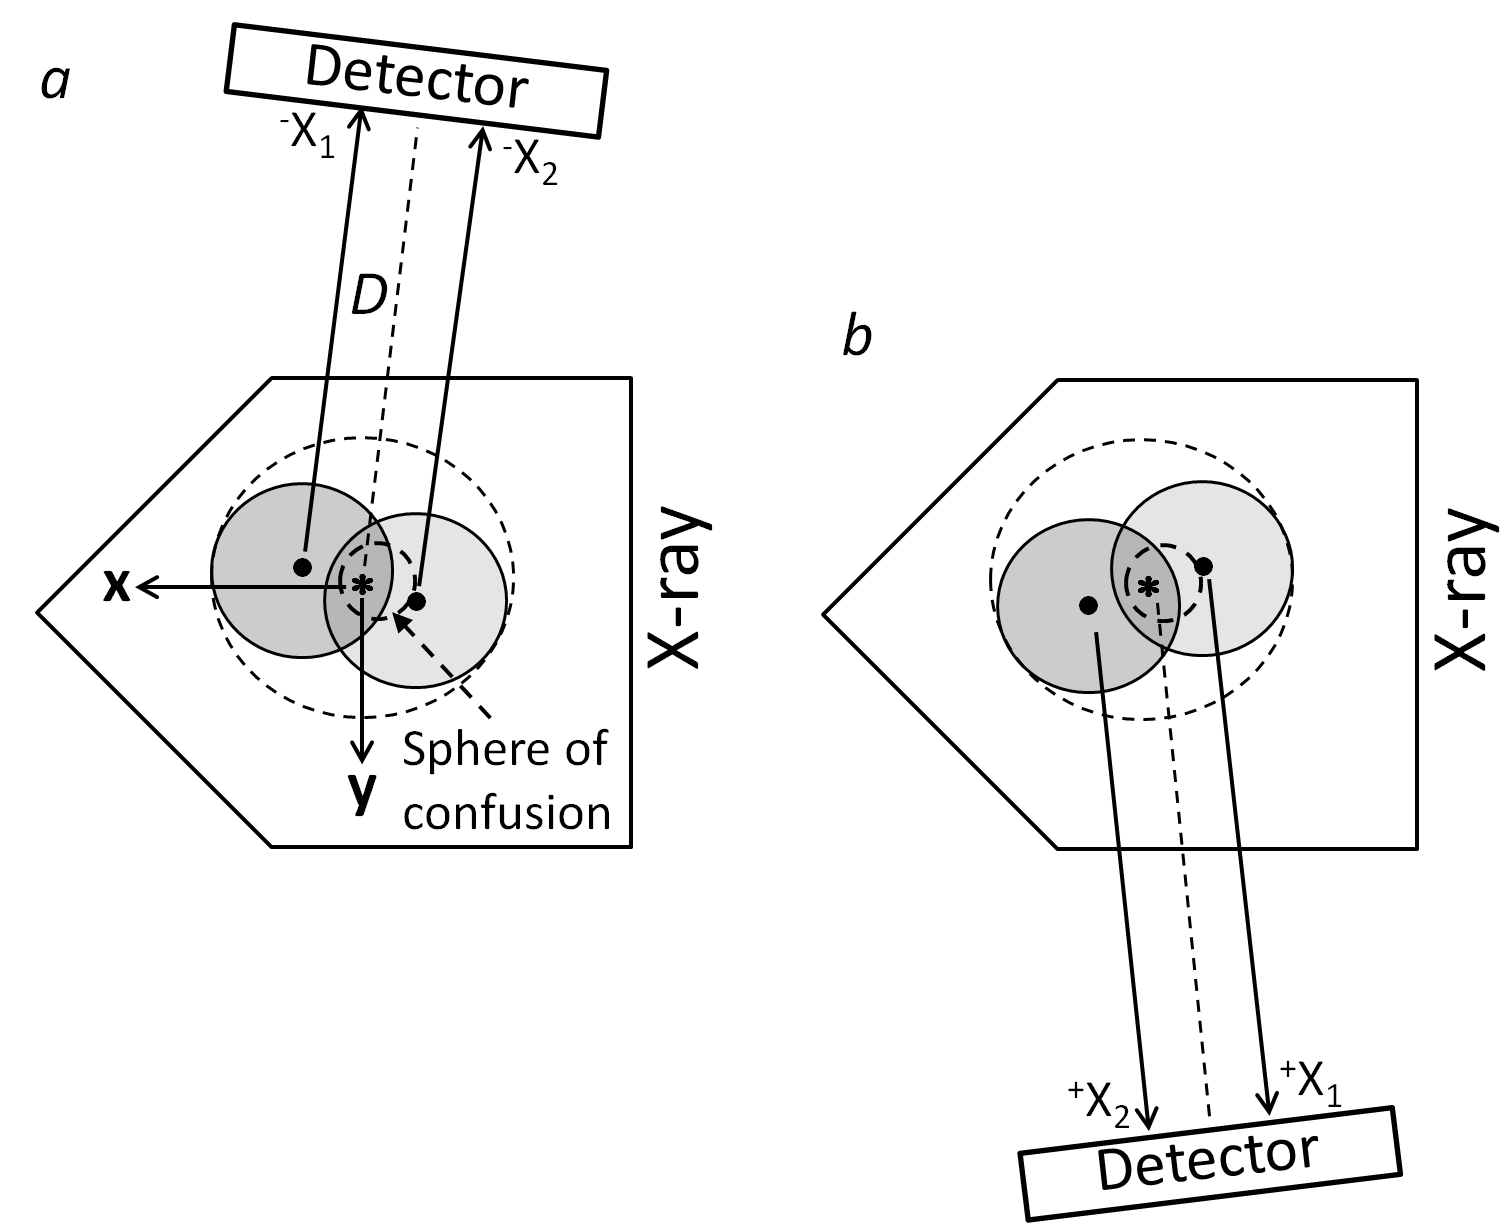
\includegraphics[width=0.8\textwidth]{eccentr.png}
    \caption{Схемы эксперимента для учета эксцентриситета образца, связанного с поворотом вокруг оси $\omega$ (ось $\omega$ идет перпендикулярно плоскости чертежа, выход показан звездочкой). $a$ --- показаны два положения образца (условные центры обозначены жирными точками), при которых проводятся съемки рефлексов и определяются положения максимумов –-- $X_1$ и $X_2$. Окружность меньшего диаметра соответствует сфере сведения, большая окружность (выделена пунктиром) ограничивает область расположения образца. Показана система координат: направление $x$ проходит через ось $\omega$ в направлении первичного пучка (условно показано, что в общем случае $x$ не совпадает с максимумом первичного пучка); $y$ --– направление перпендикулярное $x$ и лежащее в экваториальной плоскости. Направление $z$ совпадает с осью $\omega$. $b$ –-- схема для симметричного положения детектора.}
    \label{fig:eccentr}
\end{figure}

Таким образом измерение фриделевской пары позволяет использовать уточненное значение координат рефлекса
\[X_{true} = \frac{1}{2}(X + X_{frid})\]
где $X, X_{frid}$ --- координаты обычного рефлекса и его фриделевской пары соответственно.
Подставляя это в формулу~\ref{eq:bond2} получим
\begin{equation} \label{eq:bond4}
    2\theta = 2\theta_D - \frac{\gamma}{4} (X_{+} + X_{+frid} - X_{-} - X_{-frid}).
\end{equation}
\subsection{Расчет углового размера пикселя}
Зная линейные размеры пикселя $P$ и расстояние до центра детектора $D$ можно с хорошей точностью рассчитать угловой размер пикселя как
\begin{equation} \label{eq:gamma_simple}
    \gamma = \frac{P}{D}.
\end{equation}
В нашем случае $P = 135\unit{мкм}$, а расстояние $D$, указываемое прибором $D = 128.53\unit{мм}$.

Однако значение $D$, которое показывает прибор, всегда можно поставить под сомнение.
Правильнее провести калибровку положения детектора, например, согласно методике~\cite{Panchenko:2023}.
Для этого съемка эталонного монокристалла Si была проведена путем $\omega$--сканирования интервалов $10\degree$ в области углов $200\degree$ при пяти положениях кристалла по углу $\varphi$ (шаг $10\degree$).
Обработка полученных фреймов проведена по программе SearchXY~\cite{Panchenko:2023}.
В результате получено значение $D = 128.21\unit{мм}$.
Развороты детектора в наших экспериментах можно не учитывать из-за их малости и так как регистрация рефлексов проводится центральной областью детектора.

Полная калибровка занимает достаточно много времени и не всегда целесообразна.
Другой подход к определению $\gamma$ основан на съемке одного и того же рефлекса при двух угловых положениях детектора.
Так, рефлекс $\hkl(11 3 1)$ эталонного монокристалла Si был отснят при $2\theta_D = 96.4\degree, 97.0\degree$.
Смещение рефлекса $\Delta X$ позволяет провести вычисление $\gamma$ по формуле
\begin{equation} \label{eq:gamma_delta}
    \gamma = \frac{\Delta 2\theta_D}{\Delta X}
\end{equation}

Отметим, что такой подход позволяет проводить измерения при минимальных отклонениях рефлекса от центра детектора.
Полученное значение идеально совпадает с результатом, полученным по результатам полной калибровки.
Итоговое значение, использовавшееся далее
\[ \gamma = 0.06033\degree \]
\section{Обсуждение результатов}
\subsection{Изучение Si}
Измерение проводилось в нескольких переустановках образца и разных расстояниях $D$ и углах $2\theta_D$.
Также для оценки возможности использования рефлексов отстоящих от центра детектора съемка фриделевской пары $\hkl(-9 7 1)/\hkl(9 -7 -1)$ была проведена при положении детектора $2\theta_D = \pm 97.5\degree$, что является крайним положением для $D = 128.5\unit{мм}$, которое отличается от идеального почти на $0.8\degree$.
Исследование фриделевской пары $\hkl(3 -3 1)/\hkl(-3 3 -11)$ показало разницу координат $Y$ всего 4~пикс.
Среднее значение отклонение экспериментально полученных значений $2\theta$ от эталонных составило $0.0003\degree$, а среднее значение ПЭЯ отличается от эталонного на $0.0001\unit{\AA}$.
Относительная погрешность определения $d$ и ПЭЯ составила $5 \times 10^{-5}$.
\subsection{Изучение Ge}
На монокристалле Ge проводили контроль воспроизводимости установки образца и детектора.
Для этого было выполнено несколько переустановок образца, в том числе с коррекцией ориентации кристалла, изменением $D$ и угла $2\theta_D$.
При $D = 138.6\unit{мм}$ изучены рефлексы $\hkl(5 -11 -1)$ и $\hkl(1 -11 -5)$ с существенно отличными углами выведения в отражающее положение $(\varphi, \omega)$.
Для оценки возможности использования рефлексов, значительно отстоящих от центра детектора, съемка рефлекса $\hkl(7 -7 -7)$ была проведена при двух разных значениях $2\theta_D$.
Причем положение $\pm 99.9\degree$ отличалось от идеального почти на $1\degree$.
Исследование фриделевской пары $\hkl(3 -3 11)/\hkl(-3 3 -11)$ показало хороший уровень точности выведения рефлексов на экваториальную плоскость: разница координат $Y$ не превысила $\approx 7\unit{пикс.}$, что составляет $\approx 0.4\degree$.
В результате обработки профилей рефлексов были получены координаты максимумов и по формуле~\ref{eq:bond2} определены углы $2\theta$, а из них рассчитаны значения $d$ и ПЭЯ.
Среднее отклонение полученных значений $2\theta$ от теоретических составило $0.004\degree$, что соответствует точности гониометра.
Если ориентироваться на полученную величину, то относительная погрешность определения межплоскостного расстояния $\Delta d / d = 6 \times 10^{-5}$.
Таким образом, абсолютную погрешность определения ПЭЯ для Ge можно оценить как $0.0003\unit{\AA}$.
Среднее значение $a_\text{Ge} = 5.6579\unit{\AA}$ отличается от эталонного значения меньше, всего на $0.0001\unit{\AA}$.
\subsection{Изучение \YEu}
При выборе рефлекса, подходящего для уточнения ПЭЯ, мы столкнулись с проблемой оценки его интенсивности из-за хиральности точечной группы симметрии кристалла.
Так, например, теоретические значения структурной амплитуды рефлексов $\hkl(6 8 20)$ и $\hkl(8 6 20)$ соотносятся как 7 к 1.
Естественно, предпочтительно использовать наиболее интенсивное отражение.
Для решение этой проблемы предварительная съемка кристалла была скорректирована --- расстояние $D$ уменьшено до $60\unit{мм}$, а углы $2\theta_D$ увеличены до $\pm 75\degree$.
В результате были построены сечения обратного пространства, захватывающие область углов $2\theta = \range{95\degree}{100\degree}$.
Сопоставление интенсивностей рефлексов с результатами вычислений программы позволило выбрать оптимальные индексы.
По такой схеме было проведено исследование 5 монокристаллов.
Значения ПЭЯ лежат в интервале $\range{10.6902}{10.7045}\unit{\AA}$.
Разница крайних значений составляет $0.0143\unit{\AA}$.
Это значительно превосходит абсолютную погрешность определения ПЭЯ, равную $0.0007\unit{\AA}$.
Таким образом, можно однозначно утверждать, что синтезированный продукт не однороден.

Для оценки соотношения Y/Eu в изученных монокристаллах \YEu~можно использовать правило Вегарда.
Для построения соответствующей прямой были использованы литературные данные~\cite{Swanson:1954,Morris:1984}.

Для проведения РСтА расчет стратегии съемки для накопления полного массива данных производился для каждого кристалла автоматически с учетом его симметрии $(m\overline{3})$ по предварительно определенной матрице ориентации с использованием пакета программ APEX3.
Далее проводили интегрирование экспериментальных интенсивностей и вводили поправки на поглощение.
Структуры решены с помощью программы SHELXT~\cite{Sheldrick:2015:shelxt} и уточнены с SHELXL~\cite{Sheldrick:2015:shelxl} в графическом интерфейсе OLEX2~\cite{Dolomanov:2009}.
Параметры атомных смещений были уточнены в анизотропном приближении.

В результате установлено, что все изученные кристаллы изоструктурны и представляют собой твердые растворы \YEu, причем смешанными оказываются обе позиции металла.
\begin{figure}[ht!]
    \centering
    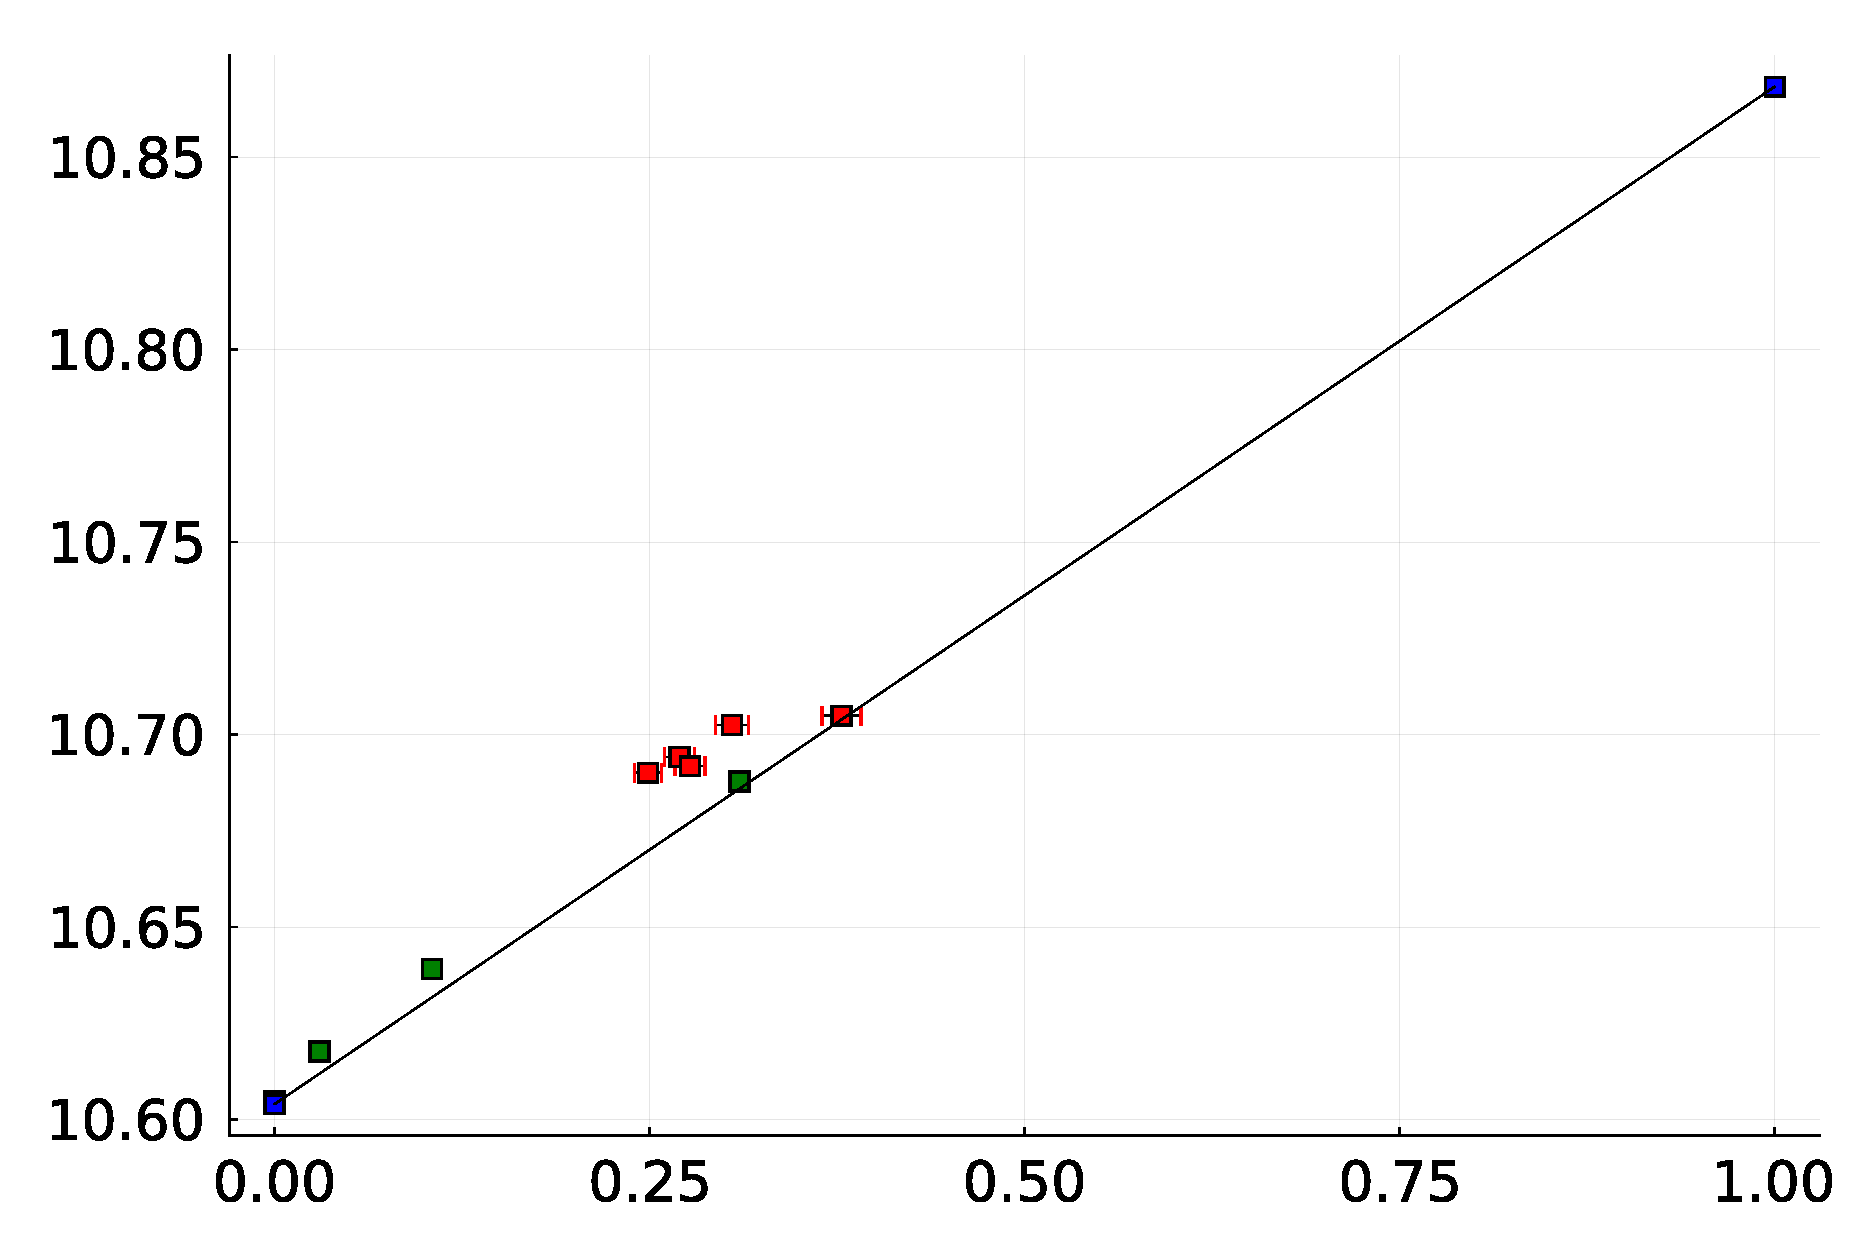
\includegraphics[width=0.8\textwidth]{YEu.pdf}
    \caption{Зависимость ПЭЯ \YEu~от мольной доли $x$.}
    \label{fig:YEu}
\end{figure}

\subsection{Оценка и учет эксцентриситета образца Si}
Несмотря на тщательную центрировку образца, в том числе с контрольными разворотами по оси $\omega$, крайне сложно точно определить его центр, особенно при неопределенной форме кристалла.
Можно ожидать, что при повороте вокруг оси $\omega$ центр образца движется по окружности, а сам образец описывает торообразную поверхность.
Подобную картину можно ожидать и при повороте образца вокруг оси $\varphi$.
Так как для использованного гониометра паспортное значение диаметра сферы сведения осей составляет $7\unit{мкм}$, центр образца при повороте вокруг обеих осей движется по достаточно сложной траектории.

Для оценки смещений центра образца при повороте вокруг оси $\varphi$, среди доступных для измерения рефлексов типов $\hkl{11 3 1}$, $\hkl{9 7 1}$ и $\hkl{9 5 5}$, было выбрано 10 вариантов, у которых значения $\omega$ лежат в интервале $\range{-82\degree}{95\degree}$.
Это примерно соответствует позиции образца при центрировании.
Все съемки проведены при одном положении детектора: $2\theta_D = -96.7\degree$, $D = 128.53\unit{мм}$.

Для оценки эксцентриситета при повороте вокруг оси $\omega$, были отобраны случаи, когда значения $\varphi$ лежат в интервале $\range{283.6\degree}{300.7\degree}$.
При этом соответствующие им углы $\omega$ лежат в интервале $\range{63.3\degree}{296.5\degree}$.
Область $\pm 60\degree$ недоступна из-за геометрических ограничений гониометра.
Графики зависимости координат от углов поворота представлены на графике~\ref{fig:eccentrSi}.

\begin{figure}[ht!]
    \centering
    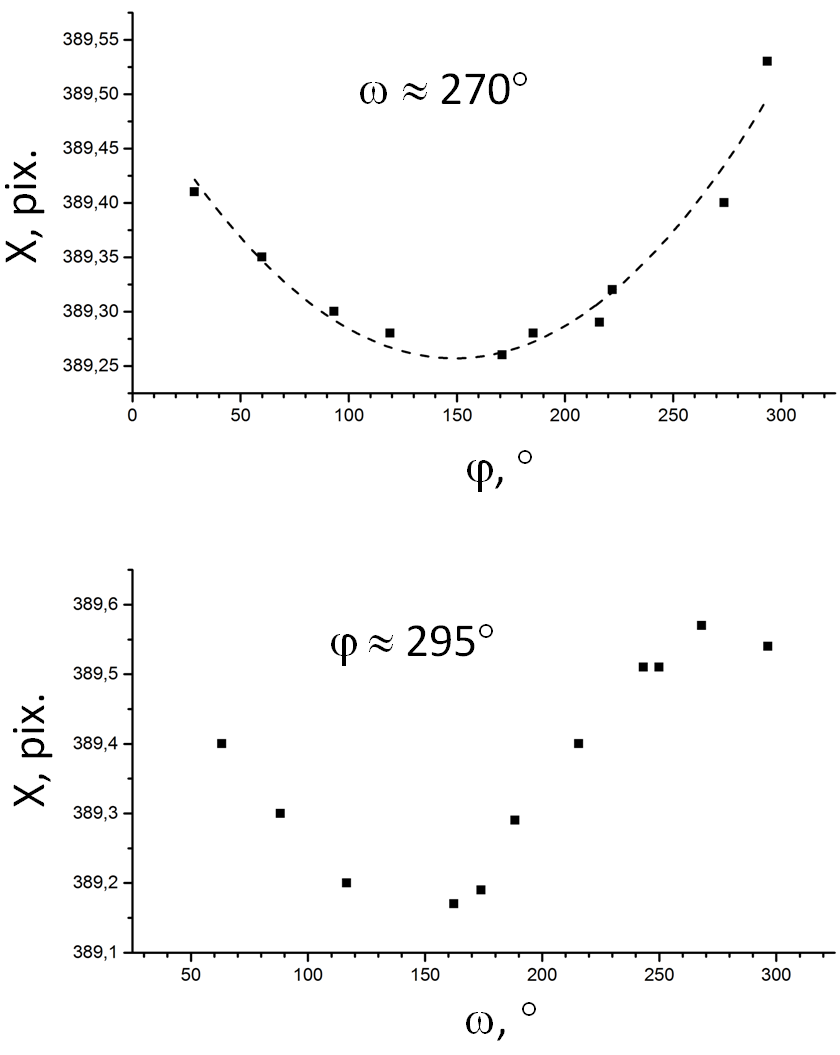
\includegraphics[width=0.8\textwidth]{eccentrSi.png}
    \caption{Смещение максимумов дифракционных отражений $\hkl(11 3 1)$, $\hkl(9 7 1)$ и $\hkl(9 5 5)$ по оси $X$ детектора из-за эксцентриситета образца: $a$ --– зависимость координаты $X$ от угла $\varphi$ (значения углов $\omega \approx 270\degree$); $b$ --- зависимость координаты $X$ от угла $\omega$ (значения углов $\varphi$ лежат в интервале от $\range{283.6\degree}{300.7\degree}$).}
    \label{fig:eccentrSi}
\end{figure}

Таким образом, проведенные два эксперимента показали одинаковую картину для эксцентриситетов, связанных с поворотами образца вокруг осей $\varphi$ и $\omega$.
При измерении ПЭЯ наиболее разумно исключить влияние именно последнего, тогда далее можно использовать подход, описанный выше~\cite{Ponomarev:1969}.

Среди всех вариантов рефлексов были выделены 5 фриделевских пар.
\subsection{Учет эксцентриситета для Si}
При произвольном выборе рефлексов расчет по~\ref{eq:bond2} приводит к значениям угла $2\theta$ в интервале $\range{96.722\degree}{96.747\degree}$.
Учет эксцентриситета по формуле~\ref{eq:bond4} уменьшает интервал значений до $\range{96.730\degree}{96.736\degree}$, а отклонения от теоретического значения не превышают $0.004\degree$.
Использование рефлексов с близкими значениями $\varphi = 66.31\degree, \, 59.35\degree$ позволяет пренебречь эксцентриситетом, связанным с поворотам вокруг оси $\varphi$.
Конечные результаты уточнения представлены в таблице~\ref{tab:Si:eccentr}.
\begin{table}[ht!]
    \centering
    \begin{tabular}{ |c|c| }
        \hline
        $2\theta$ & $96.732\degree$ \\
        $d$ & $0.47452 (3)\unit{\AA}$ \\
        $\Delta d / d$ & $6.2 \times 10^{-5}$ \\
        $a$ & $5.4311 (3)\unit{\AA}$ \\
        \hline
    \end{tabular}
    \caption{Результаты измерений ПЭЯ Si с учетом эксцентриситета.}
    \label{tab:Si:eccentr}
\end{table}

Можно отметить, что полученное значение ПЭЯ отклоняется от эталонного на $0.00006\unit{\AA}$.
Т. е. относительная разница составляет $1\times 10^{-5}$.
Еще раз подчеркнем, что результат получен лишь при частичном учете эксцентриситета, связанного с поворотом кристалла вокруг оси $\varphi$.
Чтобы полностью исключить такое влияние можно вывести одно из кристаллографических направлений вдоль оси $\omega$.
Тогда измерения можно проводить на рефлексах типа $hk0$.
При использовании трехкружного гониометра для образца такая проблема не возникает.
В нашем случае угол $\chi$ --- фиксирован, а штатные гониометрические головки предполагают только линейные смещения образца.
\subsection{Учет эксцентриситета для Ge}
Для устранения эксцентриситета, связанного с поворотом кристалла вокруг оси $\varphi$, монокристалл Ge был смонтирован на оригинальной гониометрической головке, имеющей возможность поворота образца вокруг одной оси на $\pm 10\degree$ (далее гониометрическая $\chi$--головка).
После определения ориентации кристалла были рассчитаны углы для выведения кристаллографического направления вдоль оси $\omega$. Алгоритм этого процесса описан в~\cite{Kudryavtsev:2024:eccentr}.

Расчеты для монокристалла Ge показали, что вдоль оси $\omega$ можно вывести направление $b$, так как для него значения угла $\chi = 2.2\degree$.
После поворота, исследование по нашей методике было проведено по рефлексам типа $\hkl{10 0 6}$.
Им соответствовало значение угла $2\theta = 93.943\degree$.
Все рефлексы регистрировались при одинаковых значениях угла $\varphi = -179.06\degree$.
Геометрические ограничения позволили отснять при $2\theta_D = \pm 93.9\degree$ только 12 из 16 теоретически возможных рефлексов.
При произвольных сочетаниях рефлексов значения $2\theta$, вычисленные по~\ref{eq:bond2} лежат в интервале $\range{93.935\degree}{93.958\degree}$.
Максимальные отклонения от теоретического значения достигают $0.015\degree$.
При использовании формулы~\ref{eq:bond4} углы $2\theta$ укладываются в интервал $\range{93.943\degree}{93.945\degree}$.
Отклонения от теоретического значения в таком случае не превышают $0.001\degree$.
Финальные значения для Ge представлены в таблице~\ref{tab:Ge:eccentr}.
Отклонение полученного значения ПЭЯ от теоретического составляет $0.0001\unit{\AA}$.
\begin{table}[ht!]
    \centering
    \begin{tabular}{ |c|c| }
        \hline
        $2\theta$ & $93.945\degree$ \\
        $d$ & $0.48515 (3)\unit{\AA}$ \\
        $\Delta d / d$ & $6.5 \times 10^{-5}$ \\
        $a$ & $5.6578 (4)\unit{\AA}$ \\
        \hline
    \end{tabular}
    \caption{Результаты измерений ПЭЯ Ge с учетом эксцентриситета.}
    \label{tab:Ge:eccentr}
\end{table}

Анализ координат $Y$ рефлексов Ge позволяет оценить точность выведения направления $b$ вдоль оси $\omega$.
Для этого можно построить зависимости $Y(\omega)$ для экспериментов, проведенных при дух симметричных положениях детектора $2\theta_D = \pm 93.9\degree$.
Она представлена на графике~\ref{fig:eccentrGe}.
В обоих случаях зависимости хорошо описываются синусоидами, но при $2\theta_D = -93.9\degree$ фаза сдвигается на $\theta$, а при $2\theta_D = +93.9\degree$ на $\theta + 180\degree$.
Для обработки всех рефлексов одновременно значения сдвигов вычитались из первичных значений $\omega$.
Из построенной аппроксимации следует, что максимальное отклонение направления $b$ от оси $\omega$ составляет $\approx 2.2\unit{пикс.}$, что эквивалентно $0.13\degree$.
Такое значение соответствует цене нониуса дуги гониометрической головки.
Так как отклонение лежит в ее плоскости, то можно утверждать что оно связано преимущественно с погрешностью установки угла $\chi$, а не $\varphi$.

\begin{figure}[ht!]
    \centering
    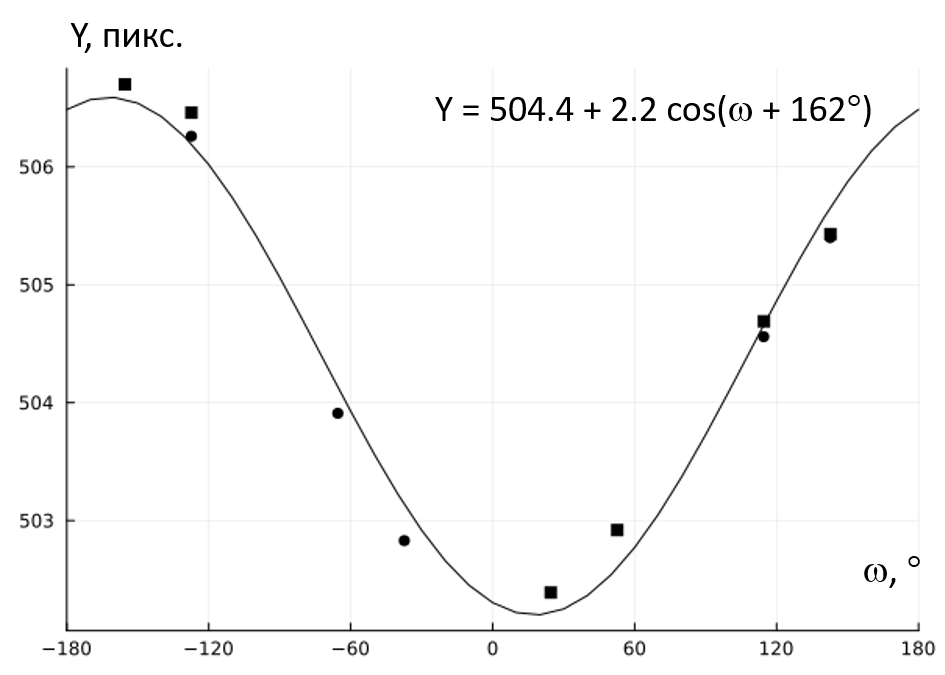
\includegraphics[width=0.8\textwidth]{eccentrGe.png}
    \caption{Зависимость координаты $Y$ от угла $\omega$ для монокристалла Ge. Для отрицательных (темные маркеры) и положительных (светлые маркеры) значениях $2\theta$ от значений $\omega$ были отняты значения $\theta + 90\degree$, тем самым позволив одновременно обработать все рефлексы. Аппроксимация функцией $Y = a_0 + a_1 \cos(\omega - \omega_1)$ выполнена с помощью МНК.}
    \label{fig:eccentrGe}
\end{figure}

\newpage
\printbibliography%

% \newpage
% \section*{Приложение}
% \begin{table}[ht!]
%     \centering
%     \begin{tabular}{ |c|c|c|c|c|c|c| }
%         \hline
%                     $hkl$ &           $D,\unit{мм}$ &  $2\theta_D, \ \degree$ &     $\varphi, \ \degree$ & $\omega, \ \degree$ &    $Y,\unit{пикс.}$ &    $X,\unit{пикс.}$ \\
%         \hline
%         $  \hkl(11 -1 3)$ & \multirow{20}{*}{128.5} & \multirow{10}{*}{-96.7} &  \multirow{2}{*}{-66.31} &                88.2 &              504.77 &              389.27 \\
%         $ \hkl(-11 1 -3)$ &                         &                         &                          &               -91.8 &              503.78 &              389.53 \\
%         $   \hkl(5 9 -5)$ &                         &                         &   \multirow{2}{*}{28.72} &                84.7 &              505.36 &              389.40 \\
%         $  \hkl(-5 -9 5)$ &                         &                         &                          &               -95.3 &              503.24 &              389.41 \\
%         $  \hkl(5 -9 -5)$ &                         &                         &  \multirow{2}{*}{119.20} &               -99.5 &              501.71 &              389.28 \\
%         $   \hkl(-5 9 5)$ &                         &                         &                          &                80.5 &              506.90 &              389.58 \\
%         $   \hkl(3 1 11)$ &                         &                         & \multirow{2}{*}{-138.01} &                97.4 &              505.92 &              389.33 \\
%         $\hkl(-3 -1 -11)$ &                         &                         &                          &               -82.6 &              502.68 &              389.32 \\
%         $  \hkl(3 -1 11)$ &                         &                         & \multirow{2}{*}{-143.63} &                84.6 &              505.92 &              389.35 \\
%         $ \hkl(-3 1 -11)$ &                         &                         &                          &               -95.4 &              502.63 &              389.29 \\
%         $ \hkl(1 -3 -11)$ &                         &  \multirow{10}{*}{96.7} &  \multirow{2}{*}{-59.35} &               -89.3 &              505.08 &              388.48 \\
%         $  \hkl(-1 3 11)$ &                         &                         &                          &                90.7 &              504.09 &              388.18 \\
%         $   \hkl(9 -1 7)$ &                         &                         &   \multirow{2}{*}{14.46} &                83.3 &              502.92 &              388.53 \\
%         $  \hkl(-9 1 -7)$ &                         &                         &                          &               -96.7 &              506.04 &              388.01 \\
%         $   \hkl(9 5 -5)$ &                         &                         &  \multirow{2}{*}{121.79} &                99.7 &              503.80 &              388.21 \\
%         $  \hkl(-9 -5 5)$ &                         &                         &                          &               -80.3 &              505.05 &              388.27 \\
%         $  \hkl(-3 11 1)$ &                         &                         & \multirow{2}{*}{-142.92} &                95.7 &              504.66 &              388.19 \\
%         $ \hkl(3 -11 -1)$ &                         &                         &                          &               -84.4 &              504.08 &              388.26 \\
%         \hline
%     \end{tabular}
%     \caption{Положения пиков $K\alpha_1$ для эталона Si.}
%     \label{tab:Si}
% \end{table}
% \begin{table}[ht!]
%     \centering
%     \begin{tabular}{ |c|c|c|c|c|c|c| }
%         \hline
%                    $hkl$ &           $D,\unit{мм}$ &  $2\theta_D, \ \degree$ &     $\varphi, \ \degree$ & $\omega, \ \degree$ &    $Y,\unit{пикс.}$ &    $X,\unit{пикс.}$ \\
%         \hline
%         $ \hkl(-6 0 10)$ & \multirow{12}{*}{128.5} &  \multirow{6}{*}{-93.9} & \multirow{12}{*}{-179.06}&              -112.4 &              503.91 &              388.61 \\
%         $ \hkl(6 0 -10)$ &                         &                         &                          &                67.6 &              504.56 &              388.47 \\
%         $ \hkl(-10 0 6)$ &                         &                         &                          &               -84.3 &              502.83 &              388.50 \\
%         $ \hkl(10 0 -6)$ &                         &                         &                          &                95.7 &              505.40 &              388.62 \\
%         $  \hkl(6 0 10)$ &                         &                         &                          &              -174.3 &              506.26 &              388.64 \\
%         $  \hkl(10 0 6)$ &                         &                         &                          &               157.6 &              506.70 &              388.74 \\
%         $\hkl(-10 0 -6)$ &                         &  \multirow{6}{*}{93.9}  &                          &              -108.5 &              502.39 &              386.91 \\
%         $  \hkl(10 0 6)$ &                         &                         &                          &                71.5 &              506.70 &              387.32 \\
%         $\hkl(-6 0 -10)$ &                         &                         &                          &               -80.4 &              502.92 &              386.82 \\
%         $  \hkl(6 0 10)$ &                         &                         &                          &                99.6 &              506.46 &              387.29 \\
%         $ \hkl(10 0 -6)$ &                         &                         &                          &                 9.7 &              505.43 &              387.21 \\
%         $ \hkl(6 0 -10)$ &                         &                         &                          &               -18.4 &              504.69 &              387.11 \\
%         \hline
%     \end{tabular}
%     \caption{Положения пиков $K\alpha_1$ для эталона Ge.}
%     \label{tab:Ge}
% \end{table}
\end{document}
